% Glava dokumenta
\documentclass[slovene, usenames,dvipsnames]{beamer}
\usepackage[utf8x]{inputenc}
\usepackage{lmodern}
\usepackage[T1]{fontenc}

% usetheme is the same as usepackage
% it just automatically prepends the 'beamertheme'
%\usetheme[]{progressbar}
\usefonttheme{progressbar}
\useoutertheme{progressbar}
\useinnertheme{progressbar}
\progressbaroptions{titlepage=normal, frametitle=normal}
\usecolortheme{seahorse}
%\usecolortheme{progressbar}

% \usetheme[sectionpage=none, subsectionpage=none, numbering=none, progressbar=frametitle]{metropolis} % izbira nastavitev oblike in barv strani
%\usecolortheme{seahorse}
\usepackage{tikz}
\usepackage[slovene]{babel}
%\usetikzlibrary{arrows}
\usepgflibrary{arrows}% for more options on arrows
\usetikzlibrary{arrows.meta}
\usetikzlibrary{positioning}
\usepackage{varwidth}
\usepackage{color}
\usepackage{amsmath} 
\usepackage{xcolor}

%\setbeamercolor{frametitle}{
%  use=palette primary,
%  bg=RoyalBlue}

%\setbeamercolor{background canvas}{
% use=palette primary,
% bg=White}

%\setbeamercolor{progress bar}{
%  fg=Blue}

%\setbeamercolor{progress bar in head/foot}{
%  fg=Red}




\uselanguage{slovene}
\languagepath{slovene}
\deftranslation[to=slovene]{Definition}{Definicija}
\usepackage{outlines}
\usepackage[document]{ragged2e}

\usepackage[customcolors,norndcorners]{hf-tikz}
\usetikzlibrary{calc} %% added

\graphicspath{{./slike/}{./slike/fazni_diagrami/}{../eps_pdf/}}
\DeclareGraphicsExtensions{.eps,.jpeg,.png,.gif,.pdf}
\usepackage[outdir=../uporabljene_slike/]{epstopdf}
\epstopdfsetup{
	suffix=,
}

\newcommand{\Alpha}{A}
\newcommand{\Beta}{B}
\newcommand{\Epsilon}{E}
\newcommand{\Kappa}{K}
\newcommand{\dif}{\mathrm{d}}

\setbeamertemplate{navigation symbols}{}
\setbeamertemplate{section in toc}[sections numbered]
\setbeamertemplate{subsection in toc}[subsections numbered]

\setlength{\abovedisplayskip}{0pt}
\setlength{\belowdisplayskip}{0pt}

\author{Jure Lapajne}
\title{Calculation of nmr parameters in paramagnetic metal-organic materials}

\begin{document}
\maketitle

\begin{frame}{Presentation plan}
  \begin{enumerate}
  \item NMR --- what and why \pause
  \item MOFs = Metal---organic frameworks \pause
  \item NMR parameter calculation \pause
  \item DFT \pause
  \item Preliminary results \pause
  \end{enumerate}
\end{frame}

\section{NMR}
\begin{frame}{Nuclei and external magnetic field}
  \begin{itemize}
  \item strong external magnetic field: several T
  \item nuclei with magnetic moment: lowest energy state splits
    \item two new states $\Delta E$ apart
  \item radio frequency spectrum: excitations from low to high energy states
  \item absorption peak at $\Delta E=\hbar \omega_{res}$
    \item $\omega_{res}$ depends on $B_{eff}(observed nucleus)$
    \end{itemize}
    \begin{minipage}[]{\textwidth}
      \centering
    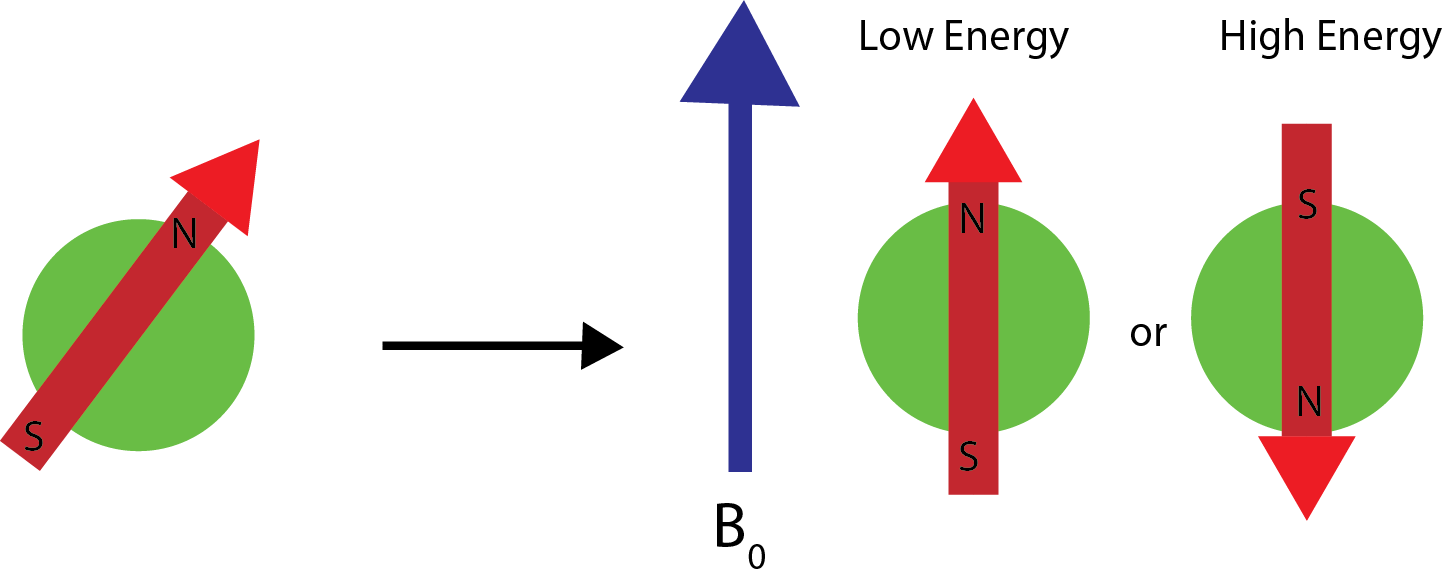
\includegraphics[width=0.5\textwidth]{spin_energy_states.png}
\end{minipage}
\end{frame}

\section{NMR}
\begin{frame}{}
  Several parameters affect $B_{eff}(nucleus)$ and $\omega_{res}$:
  \begin{itemize}
  \item electronic structure -- shielding of external magnetic field 
  \item spin--spin coupling to nearby nuclei and unpaired electrons
   \item unpaired electrons: large paramagnetic shifts
    \end{itemize}
\end{frame}

\end{document}